\documentclass[10pt,twoside,openright,a4paper,twocolumn]{book}

\usepackage{factions}
\usepackage{lipsum}

\title{Fractured Kingdom}
\subtitle{A Dungeons \& Dragons (5th Edition) Campaign Setting}
\author{Daniel P. Wright}

\begin{document}

\pagenumbering{gobble}

\newgeometry{margin=1in}
\begin{titlingpage}
\factionstitle
\end{titlingpage}
\restoregeometry

\frontmatter
\pagenumbering{gobble}

\onecolumn
\thispagestyle{empty}
\null\vfill
\begin{flushleft}
\textit{Fractured Kingdom}

{\textcopyright} 2015 by Daniel P. Wright.

\bigskip

{\ccLogo} {\ccAttribution} {\ccShareAlike}

This work is made available under a Creative Commons Attribution-ShareAlike 4.0 International License.

See \url{http://creativecommons.org/licenses/by-sa/4.0/} for more information.
\end{flushleft}
\twocolumn

\cleardoublepage

\tableofcontents

\thispagestyle{empty}

\mainmatter

%\part{An adventurer's guide to Sabilia}

\chapter{Creating and playing a character in \textsc{Fractured Kingdom}}
\label{chap:character-creation}

\lettrine{W}{\textit{elcome}} \textit{to the world of Tiermea! Or, to be more
specific, to the Kingdom of Sabilia, the greatest and most ancient of
civilisations ever to grace the land!  Come, step forth and show yourself!
From what House do you hail?  Are you a Gilhall or a Lanstone; a Pearbrandt or
a Lindwell?  No matter, come, come!  Step inside, and let me show you
around\dots}

\textsc{Fractured Kingdom} is a campaign setting for the Dungeons \& Dragons
\ordinalnum{5} Edition roleplaying game.  It takes place in a world of high
intrigue, where ancient dynasties fight for control of the Kingdom by whatever
means necessary, where the fates of men are as likely to be decided by the
contents of a letter as in the field of battle.

This booklet will tell you all you need to know in order to start playing a
character in the world of \textsc{Fractured Kingdom}.  The setting is, by and
large, similar in style to the standard high fantasy worlds of \textit{Dungeons
\& Dragons}, so this document will focus only on those areas which deviate from
that, or where more detail would be helpful.  For more information about the
standard character creation process, please refer to the \textit{Player's
Handbook}.

\begin{figure*}[ht]
  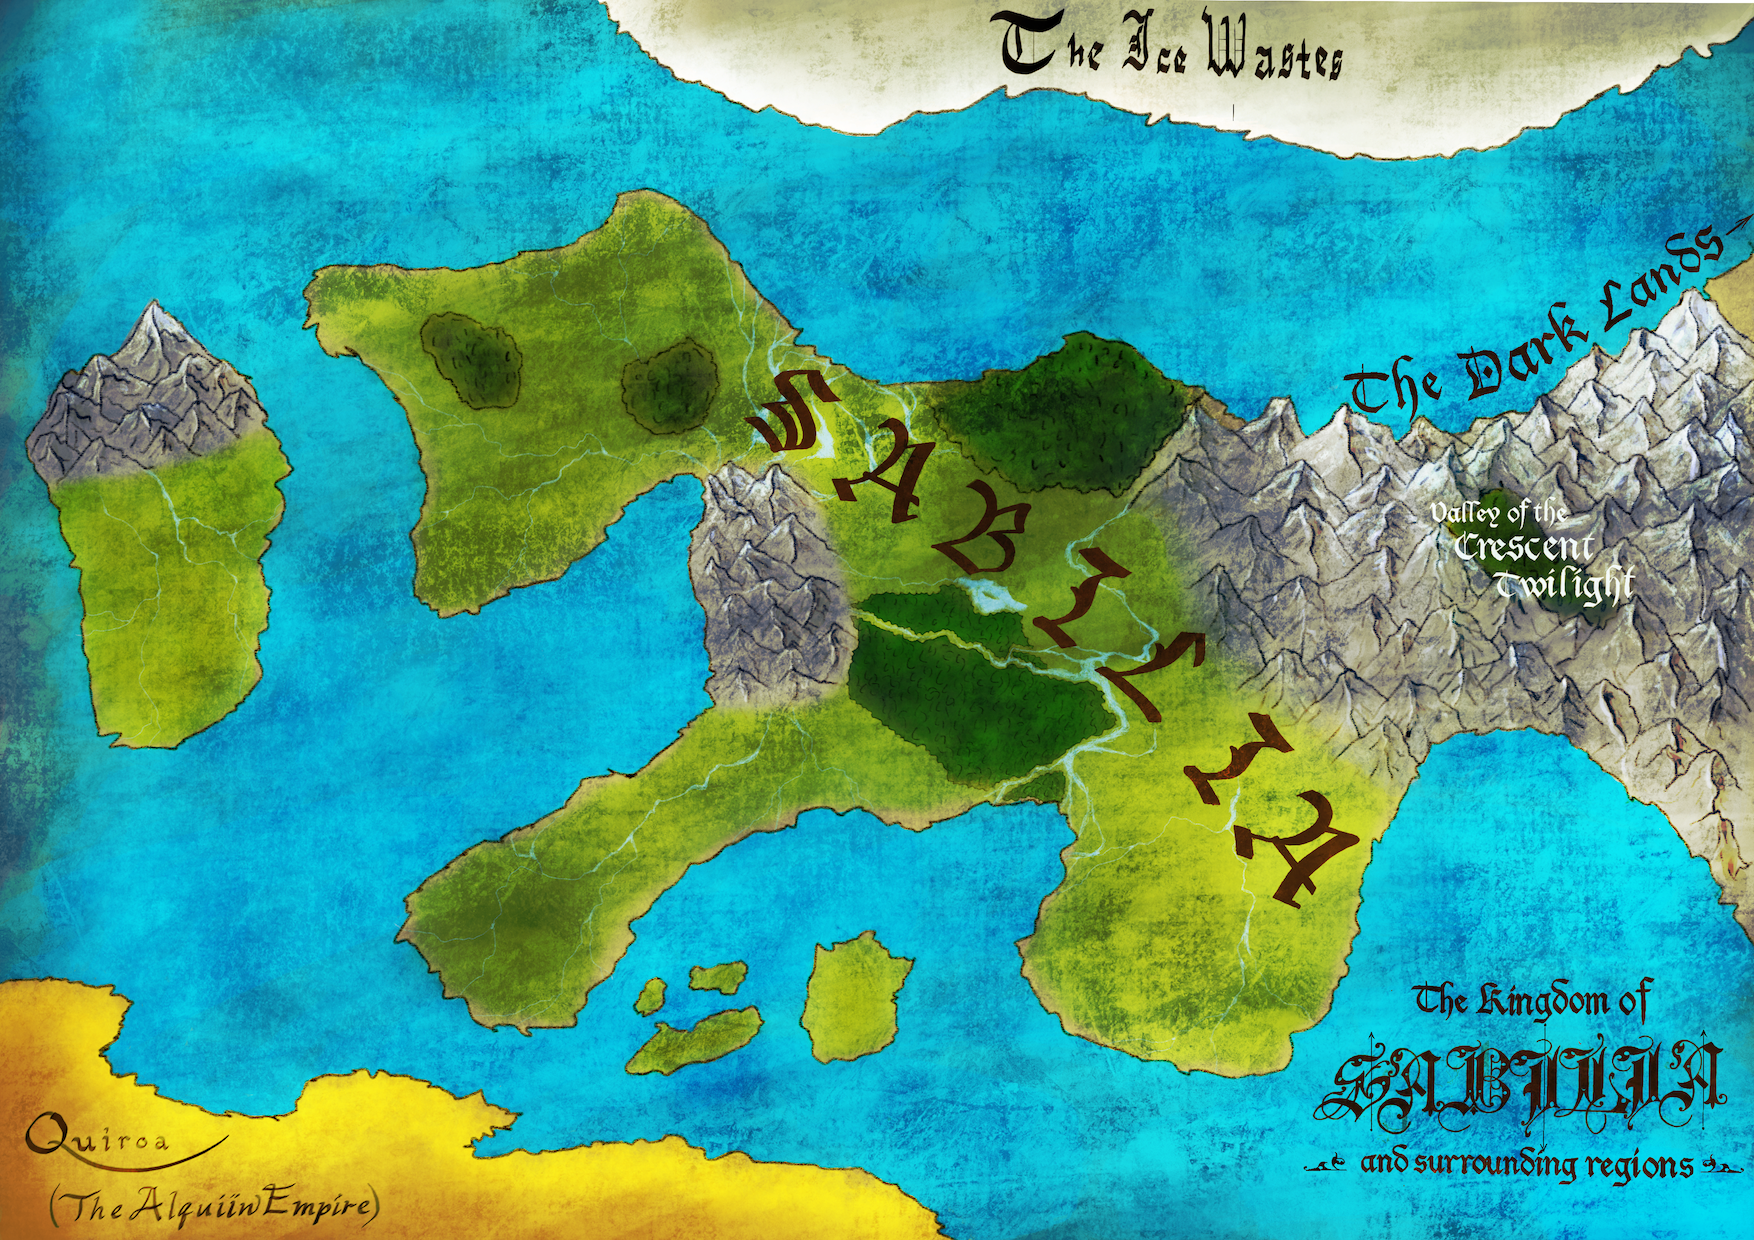
\includegraphics[width=\textwidth]{images/ferroa-map.png}
\end{figure*}

\section{Sabilia in Summary}

Adventures take place in the Kingdom of Sabilia, a state which occupies the
majority of the landmass of Ferroa, in the world of Tiermea.  Sabilia is a
large and somewhat inward-looking Kingdom composed of a number of dynasties,
who after centuries of fighting have settled into a somewhat uneasy tolerance
of one another.  Chief among these dynasties are the Airnsim, from whom the
Kings and Queens of the land have, for the most part, been drawn.

The Kingdom was founded, it is said, back in the First Days, when the gods
walked amongst men.  Each of the great dynasties traces a line back to one
of these gods, and their power flows directly from this divine heritage.

However, the gods left Sabilia.  First they departed the land, but remained in
spirit, as gods do\dots but eventually they left completely, leaving the people
of Sabilia to fend for themselves.  Some believe they will return, and the
priesthood continues to practice their devotion while they wait.  Others
believe the gods have abandoned the land completely, and left the people in the
hands of their offspring.  The gods, absent, have remained silent.

To the East of Sabilia lie the Eastern Peaks, in which is nestled the Valley of
the Crescent Twilight, a relatively small state which is independent of Sabilia
and which is viewed by Sabilians with a kind of curious exoticism.  Beyond the
Eastern Peaks lie the Dark Lands, where it is always night and monsters roam.
Few who have ventured there have ever returned.

South of Sabilia and across the Middle Sea is the other major world power, the
Alqui{\"i}n Empire.  The Empire is rumoured to hold sway over the whole of the
vast continent of Quiroa, though few Sabilians travel beyond Quiroa's coastal
trading towns and the general perception in Sabilia is that it is mostly desert
anyway.

\section{House Allegiance}

Perhaps the most important thing to consider when creating a character for
\textsc{Fractured Kingdom} is the House with which you are aligned.  You do not
necessarily have to be a member of one of the great lineages: you may be a
servant in their employ; a peasant on their lands; a trader in their ports; a
knight in their army; or any manner of other things.  But all children born
into Sabilia are born within the borders of one of the Great Houses, and they
know their heritage as surely as they know whether they are Human or Elf.

House alignment becomes more rigid as your position in society rises.  A lowly
peasant may slip across the border into a neighbouring region and escape
notice; within two or three years they will be completely assimilated.  A
Lord's daughter, on the other hand, cannot escape the duty she bears her House
except by marriage or war, which in the best case will lead to her owing that
same duty to another House and in the worst, destitution.

More information about each of the Great Houses can be found in
\autoref{chap:houses}.

\section{Social Rank}

Social rank plays a large role in Sabilia, both in terms of how you are treated
and in what you can achieve.  The Sabilian Kingdom is a highly structured,
deeply divided society, where it is very unusual for the aristocracy to mix
with the common folk, and there is very little scope for self-improvement or
movement within the class hierarchy.

An ambitious few do manage it---usually through an an accumulation of wealth
and influence which allows them to rise above their usual status.  Still,
memories in Sabilia are old, and even after a few generations the Great Houses
may still view them as ``new money''.  Of course, while an ambitious Lord may
be granted land or titles his name will never be listed amongst the Great
Houses, for the blood of the gods does not run in his veins.

Players can choose to play characters of any social rank, from the lowest
peasant to the greatest lord.  That said, some characters may be more suited
to a particular campaign than others; a game of high-level political intrigue,
for example, would be harder to play as a village leatherworker.  If you are
in doubt as to how well your character would fit in, consult your Dungeon
Master for advice.

\section{Class}

Class choice in \textsc{Fractured Kingdom} is much the same as that described in
the \textit{Player's Handbook}, with the following caveats:

\begin{description}
\item [Cleric] is not a valid choice of class. It is not that Sabilia has no
clerics; it does, but since the gods have left the land they have no power and
thus can cast no spells.  If you want to play an adventurer priest, you should
choose another class (such as Fighter or Rogue), and choose the Acolyte
background.

\item [Monk] is only valid for characters coming from the Valley of the
Crescent Twilight, or those who may have trained there.  Both are very rare
occurrences in Sabilia, so whether to allow them is at the discretion of the
Dungeon Master.

\item [Paladins] in Sabilia have the divine blood of one of the Great Houses
flowing in their veins, from which they get their power.  They must also have
received martial training in order to reach their Paladin status.  For this
reason, they must be members of the nobility.

\item [Sorcerors] get their power from the same divine source, but in their
case it has transformed somehow.  They must be blood relations with one of the
great dynasties, but as they require no martial training they don't have to be
members of the aristocracy; they might be the illegitimate offspring of some
part of the nobility, or have some other less well-understood link.  They may
well be unaware of their blood relation when their power begins to manifest.
Either way, sorcery is viewed with great suspicion in Sabilia, so noble and
common sorcerors alike will try and hide the fact.
\end{description}

\noindent
The lack of a Cleric class will come as a shock to those used to having Cleric
as the standard healing class of an adventuring party, and indeed it does
change the balance of a group.  Parties looking for a healer would do well to seek
out a Paladin, Ranger, or Bard, all of which have access to healing magic.

\section{Race}

Sabilia is an overwhelmingly Human nation, with a couple of pockets of the
Kingdom where Dwarves or Elves are more common.  Half-Elves are unusual but do
exist, mostly in the domain of House Gilhall.  Similarly, Halflings are mostly found in
the regions of House Lindwell, and since they rarely venture abroad they aren't often
seen elsewhere.  More information about which races are common in different areas
of the Kingdom can be found in the descriptions of each of the Houses in
\autoref{chap:houses}.

Gnomes, Dragonborn, and Tiefling do not exist in Sabilia and thus it is not
possible to play them.  Sabilia does have the odd infestation of goblins, orcs,
and similar creatures, so it is not inconceivable that a Half-Orc could exist,
but they would encounter such a huge amount of discrimination in life (if they
weren't simply killed at birth) that it is highly recommended not to play them,
and whether it is even available as a choice is at the Dungeon Master's
discretion.

\section{Languages}

The principle language used in Sabilia is Sabilian, which fills the role of the
Common tongue referred to in the \textit{Player's Handbook}.  The race-specific
languages such as Elvish, Dwarvish, Halfling and so on work exactly as standard.
As well as those, the following languages are also spoken in some parts in and
out of the Kingdom:

\begin{description}
    \item [Old Sabilian] is the ancient language from which Sabilian is derived,
said to be the original language of the gods.  In ancient times, Sabilia was host
to a whole range of languages, but Old Sabilian was the standard for formal
written language.  It is not used at all in modern times except in certain religious
rituals.
    \item [Fluminis] is a somewhat obscure language spoken up and down the
rivers of the Marshrance region.  It has no written form, and has survived the
centuries of Sabilian standardisation because it is the language in which the
ancient tales of the Marshrance House are told in their lands, through stories
handed down the generations, to songs performed by their bards.  Most of
of those who grow up in Marshrance are bilingual, and switch easily between
Fluminis and Sabilian in conversation.
    \item [Quiroan] is the common tongue spoken on the continent of Quiroa.
It is not widely spoken in Sabilia, just as Sabilian is not widely spoken in Quiroa,
but traders living on the coast may have learned a little.  The language has a delicate,
flowing script, and a long history of literature and science---for those Sabilians
sophisticated enough to study it.
    \item [Y\=ugrese] is the language of the Valley of the Crescent Twilight.  It
is a tonal language which, like Elvish, has a musical ring to it.  Other than that there
is no relation between the two languages, or indeed between it and any other
known language.  The Valley's isolated location has no doubt encouraged this
entirely independent linguistic evolution.
\end{description}


\chapter{The Great Houses of Sabilia}
\label{chap:houses}

\begin{figure*}[ht]
  \includegraphics[width=\textwidth]{images/sabilia-political.png}
  \centering
  \textit{Political map of the Sabilian Kingdom}
\end{figure*}

\lettrine{F}{orged} by the gods, tempered by war; bound through marriage and
ruptured by betrayal; the Great Houses form the spine on which hangs the Kingdom
of Sabilia.
Their heroes are legends, admired by peasants and nobles alike.  In their histories,
our future is written.  They are both the foundation of tradition in these lands,
and the spring from which flows all political power.  They are the core that holds
this Kingdom together; and the flaw that, one day, will rip it apart.

It is said that the Houses sprung forth from the gods themselves, in the First
Days when gods and men roamed the earth together.  Thus in the blood of the
nobility runs the blood of the gods, and in their hands lies the fate of the
Kingdom.  It is not known why the gods left Tiermea, but when they did they
left the Great Houses as heirs to their land and, ultimately, executors of
their will.

\section{The Majestic Houses}

Since ancient times, the greatest of the Great Houses have been the noble House
Airnsim, and its two lesser branches, Houses Gilhall and Pearbrandt.  Whether
it is their Elven ancestry or their quiet, fair-minded approach to rulership,
these Houses are admired by their people and respected by their peers.

\subsection*{House Airnsim}

\begin{wrapfigure}{R}{0.4\columnwidth}
  \includegraphics[width=0.38\columnwidth]{images/HouseAirnsim}
\end{wrapfigure}

\begin{description}
\item[Motto] \textit{Strength through purity}

\item[Symbol] An unadorned circle

\item[Racial Makeup] High Elf
\end{description}

\noindent
The oldest and most revered of the Great Houses, House Airnsim has long been
that from which the Kings and Queens of Sabilia were drawn.  Members of House
Airnsim consider all the other Houses to be equal and beneath them, which
though a rather arrogant outlook allows them to rule with very little bias.

One of the reasons for this belief is the purity of their High Elf bloodline.
House Airnsim believes High Elves to be fundamentally superior to the other
races, and as the purest Elven line which can trace its origins back to the
gods themselves, they are naturally superior amongst Elves.

For this reason, House Airnsim does not intermarry with other Houses, a fact
which has caused more than a few raised eyebrows in some of the more tawdry
areas of lower society.  Inter-House or interracial romances are thus treated
as a great scandal, and those members of the Airnsim nobility who indulge in
them are summarily disowned and made unwelcome in their homeland.

\subsection*{House Pearbrandt}

\begin{wrapfigure}{R}{0.5\columnwidth}
  \includegraphics[width=0.48\columnwidth]{images/HousePearbrandt}
\end{wrapfigure}

\begin{description}
\item[Motto] \textit{Carpe fortuna}

\item[Symbol] An ancient coin

\item[Racial Makeup] Human
\end{description}

\noindent
House Pearbrandt hails from the coastal areas in Sabilia's Southern regions,
where the land juts out toward Quiroa.  Because of this enviable position they
have a long history of trade with Quiroa, making them one of the richest
families in the Kingdom.  The cities they control tend to be a little more
cosmopolitan then the rest of Sabilia as people from all walks of life travel
their to find their fortune.

The members of House Pearbrandt look on their haughty Elven neighbours with a
sense of amused tolerance, believing that the fortune they've amassed over the
generations far outweighs any notion of ``bloodline purity''.  Although they
find the Airnsim attitude to be a little condescending, they generally get
along, and so long as the Elves don't start poking their noses into their
business affairs House Pearbrandt pays them a grudging respect.

\subsection*{House Gilhall}

\begin{wrapfigure}{R}{0.5\columnwidth}
  \includegraphics[width=0.48\columnwidth]{images/HouseGilhall}
\end{wrapfigure}

\begin{description}
\item[Motto] \textit{Truth and Beauty}

\item[Symbol] A fallen leaf

\item[Racial Makeup] Wood Elf, Half-Elf, Human
\end{description}

\noindent
House Gilhall traces its origins back to House Airnsim, from which it
originated thousands of years ago.  The tale of its progenitor, Lord Faellwyn,
is often recounted in the Gilhall Court.  He was a prince of the House Airnsim,
the heir and first in line, when he committed the unforgivable crime: he fell
in love with a Dryad called Sylwyr who inhabited the nearby Gilwood Forest.  He
ran away from the Estate and built Gilwood Hall in the centre of the Forest,
where he married Sylwyr and founded House Gilhall.

From their loins sprang the race of Wood Elves, who went on to mix freely with
the surrounding Humans as well as any further runaways from House Airnsim.  To
this day the lands of House Gilhall are known as a place of tolerance and
appreciation for the finer arts, and lovers often choose Gilwood Forest as
their destination when they decide to elope.

For their part, House Airnsim denies the story, claiming that Lord Faellwyn was
never a member of the Airnsim family, that he is mentioned nowhere in their
records (which are generally long and detailed), and the history is likely a
myth invented to improve the image of the mongrel Wood Elves in the eyes of the
common folk.  Relations between the two houses are polite but fragile---though
they have counted each other as allies for many centuries now, Elven memories
are long, and occasionally old wounds flare up and they find themselves bitter
enemies once more.

\section{Houses of the Crooked Isle}

The Crooked Isle lies to the West of the Sabilian mainland, separated by the
narrow and pirate-infested Channel of Daggers.  There are two Houses that make
their home there, though they have little to do with one another---the
honourable House Lanstone and the devious House of Calbrand.

\subsection*{House Lanstone}

\begin{wrapfigure}{R}{0.5\columnwidth}
  \includegraphics[width=0.48\columnwidth]{images/HouseLanstone}
\end{wrapfigure}

\begin{description}
\item[Motto] \textit{Order breeds honour}

\item[Symbol] An anvil and hammer

\item[Racial Makeup] Dwarf
\end{description}

\noindent
Occupying the mountains to the North of the island is the stern House Lanstone.
After Airnsim, Lanstone is said to be the oldest name in Sabilia.  The Dwarves
who make up its people, it is claimed, rose fully-formed from the ground, born
of the very rocks themselves.

If the noble line is forged from rock, so too are the attitudes of its citizens.
The Lanstones are a hard, traditionally-minded people, who believe there is a
correct way to do things, and who strive to follow that correct path.  That
said, they are not an arrogant people. Unlike the Airnsim, they do not believe
in the superiority of any one race or House.  Tradition and order, they say, is
at the root of all morality.  That is the one true path to righteousness, and
anybody may follow it who so choose.

\subsection*{House Calbrand}

\begin{wrapfigure}{R}{0.5\columnwidth}
  \includegraphics[width=0.48\columnwidth]{images/HouseCalbrand}
\end{wrapfigure}

\begin{description}
\item[Motto] \textit{Respect. Blood. Power.}

\item[Symbol] A fish-hook

\item[Racial Makeup] Human
\end{description}

\noindent
Scattered across the remainder of the island are the scions of House Calbrand.
Rather than one large estate managing the whole of their territory, House
Calbrand is made up of a number of smaller regions, each managed by one of
Lord Calbrand's twelve children.

The Crooked Isle is known as a haven for criminal activity in Sabilia, and for
generations it has been rumoured that House Calbrand is actively involved with
this activity, though no direct link has ever been proven.  It is undeniable,
though, that the criminal networks across Sabilia can all trace their roots to
this one corner of the Kingdom.  Calbrand must be either complicit or
incompetent, say the other Houses---behind closed doors, of course, for fear of
retribution.

\section{Houses of the Westlands}

The Westlands comprise the largest contiguous region in Sabilia in terms of
landmass.  They stretch from the coast of the Channel of Daggers, where House
Balmour keeps a strict watch for pirate activity, around the top of the Western
Alps, after which House Marchrance borders with Houses Gilhall and Valenguard.
To the North, House Lindwell tend their relatively peaceful lands and do what they
can to stay out of trouble.

\subsection*{House Balmour}

\begin{wrapfigure}{R}{0.5\columnwidth}
  \includegraphics[width=0.48\columnwidth]{images/HouseBalmour}
\end{wrapfigure}

\begin{description}
\item[Motto] \textit{Only total victory will suffice}

\item[Symbol] Crossed swords

\item[Racial Makeup] Human
\end{description}

The most competitive of the Great Houses is House Balmour.  They boast
some of the finest military prowess in the Kingdom; a result of the highly
regimented culture and lifestyle within their lands.  All boys learn the martial
arts as part of their schooling, and many dream of becoming a Sabilian
Champion.

Every year, House Balmour hosts the Sabilian Games, a tournament to find
the most celebrated champions in all the land.  There are contests of magic
and cunning, but by far the most popular events are the physical bouts---fencing,
jousting, and archery.  The Games' finale takes place when the winners
of each of these three events are pitted against each other in a mounted
three-way battle, the outright winner of which is dubbed that year's Sabilian
Champion.  Many of the champions returned by the contest have been from
House Balmour itself or its lands, a fact in which they take much pride.

Unofficially, there is also a bareknuckle fisticuffs contest which, although
strictly illegal, attracts a great number of spectators every year.  This underground
tournament, dubbed the Sabilian Fists, or just the Fists, is strictly the domain
of the lower classes, and it would be a great scandal for the nobility to be caught
watching it, much less competing!  Nevertheless, it is an open secret that they
often do watch, and the organisers do their best to accommodate their desire for
anonimity since they bring so much money to the betting-houses.

\subsection*{House Lindwell}

\begin{wrapfigure}{R}{0.5\columnwidth}
  \includegraphics[width=0.48\columnwidth]{images/HouseLindwell}
\end{wrapfigure}

\begin{description}
\item[Motto] \textit{A simple life is a peaceful one}

\item[Symbol] A hoe and scythe

\item[Racial Makeup] Human, Halfling
\end{description}

The lands of House Lindwell sit snugly between those of Houses Balmour
and Marshrance, sheltered from the treacherous seas to the West and the
lawless mountains to the South.  As a result its people are a quiet, unassuming
folk, whose ambitions rarely extend beyond making a good living for their
families and saving enough to enjoy a quiet retirement.  They have a
reputation throughout the Kingdom for honesty and openness, but also for
na{\"i}vet{\'e} and innocence.

Like the people, their leaders are not inclined to impose.  None of the Kings
in the history of Sabilia have been drawn from House Lindwell, and in
general they prefer not to involve themselves in the diplomacy and intrigue
of political life.  They regard their primary concern to be to their people, and
strive to raise taxes fairly and offer support where needed.

Despite their lack of ambition, the people of House Lindwell have courage
where it counts. It is rarely by choice that they venture beyond the Lindwell
borders for a life of adventuring, but having done so they will defend their
companions through the most dire circumstances.

\subsection*{House Marshrance}

\begin{wrapfigure}{R}{0.5\columnwidth}
  \includegraphics[width=0.48\columnwidth]{images/HouseMarshrance}
\end{wrapfigure}

\begin{description}
\item[Motto] \textit{Never stay still}

\item[Symbol] A decorational rose

\item[Racial Makeup] Human
\end{description}

House Marshrance makes its home amongst the network of rivers and marshlands
North-East of the Western Alps.  The region operates as a loosely federated
collection of clans, some of which trace a direct lineage to House Marshrance
itself, while others are without noble blood---though outsiders would struggle to
tell the difference.  The distinction between nobleman and commoner is less marked
here than elsewhere; no matter their status, most people of the Marshrance region
live aboard narrowboats which travel the waterways, or, in the drier Eastern regions,
as part of travelling caravans.  Decisions which affect the region are decided at vast
moots, where all have the right to speak.  That said, the final decision on such matters
does still lie with the Rivermaster, Lord Marshrance, who leads the moot and weighs the opinions of his people before casting judgment.

Apart from their obvious affinity with water and horses, House Marshrance has a
reputation for sorcery and trickery.  Many of those who travel out of the region make
their living telling fortunes or entertaining with music and magic tricks.  It is said that
there are some who can commune with the dead, though most Marshrance folk would
be quick to tell you that that is an old, outdated prejudice.

\section{The Border Houses}

To the East of Sabilia lie the Border Houses, pressed up against the Eastern
Peaks.  These two valiant Houses have protected Sabilia over the centuries from
raids led by creatures from the Dark Lands.  Their service to the Kingdom is
appreciated by those who do not have to worry about such things, though their
proximity to the Dark Lands has left them with a somewhat sinister mien, which
sometimes leads the Western folk to view them with suspicion.

\subsection*{House Raventomb}

\begin{wrapfigure}{R}{0.5\columnwidth}
  \includegraphics[width=0.48\columnwidth]{images/HouseRaventomb}
\end{wrapfigure}

\begin{description}
\item[Motto] \textit{Wisdom and grace}

\item[Symbol] A single tear

\item[Racial Makeup] Human
\end{description}

\noindent
House Raventomb is unique among the Great Houses in that the title is passed
down not through a direct blood lineage, but through adoption.  Centuries ago,
the Lady Raventomb swore that she would take no husband, and instead adopted
a daughter from the priesthood to take her place when she was gone.  This
tradition has continued, so that since that day there has never been a Lord
Raventomb.

For this reason the priesthood remains strong despite the gods having left
Sabilia.  Families send their firstborn daughters to study there, in the hope
that they might be selected to rule the Raventomb domains in the future.  Even
if they are not selected, they are given the best education and often leave the
priesthood well prepared to take on important roles in local governance or
diplomacy abroad.

Raventomb is a very agricultural area, so the remaining sons and daughters of a
household will generally be put to work raising livestock or plowing fields.

The reason for Lady Raventomb's oath remains shrouded in mystery.  Some say she
was once married, and that her husband betrayed or spurned her, leading her to
abandon men altogether.  Others say he died, and call her the Raventomb Widow.
Yet others say she never took any man, but that her devotion to her people was
so strong that she surrendered herself to their service.  Whatever the reason,
Raventomb certainly reaps the benefits of its unusual system.  The generally
high quality of education means that many of the most powerful figures in
history have originated from the area, while the strong agricultural base grows
enough food to feed half of Sabilia.

\subsection*{House Valenguard}

\begin{wrapfigure}{R}{0.5\columnwidth}
  \includegraphics[width=0.48\columnwidth]{images/HouseValenguard}
\end{wrapfigure}

\begin{description}
\item[Motto] \textit{Constant vigilance}

\item[Symbol] A portcullis

\item[Racial Makeup] Human
\end{description}

For centuries, House Valenguard has acted as the last line of defence between
the Kingdom of Sabilia and the horrors in and beyond the mountains; the
creatures of the Dark Lands.  They are brought up on a strict military regimen,
and their first priority is protection of the Kingdom.

While they take their rôle as protectors very seriously, those from other
regions vary in how they view the people of House Valenguard.  Some of them see
them as overly cautious, or stuck reliving former glories.  Most of them have
never had to face the creatures which sometimes emerge from the Dark Lands.
Some even intimate that they don't exist; that they are simply figments of the
Valenguard's imaginations.  Those of House Valenguard, of course, would respond
that the reason they have never seen these creatures is that they were stopped
at the frontier.

The reality is probably a mix of the two.  The old tales speak of fierce
monsters; of demons and dragons emerging from the mountains and raining fire
down on the lands of Sabilia.  The truth is that most of the forces House
Valenguard have had to drive away recently are a lot more petty than that.
There are those that believe that the demons are simply lying in wait, biding
their time until they can come in full force and overrun the kingdom.  Most
dismiss this as paranoid rambling, but those of House Valenguard do not.  Even
if they don't think it is likely to happen in the near future, they remain
vigilant---just in case.

\end{document}
